% 原文 p.88（後半）


\subsectionlink{デコヒーレンスの単純な模型}
Zurekが1982年に初めて導入して研究した模型\cite{ref009}を用いて、環境誘起デコヒーレンスと超選択の、基本的な特徴と力学を説明しよう。この模型はかなり容易に解けるので、第3章と第5章で論じる、より複雑なデコヒーレンス模型への、よい導入となる。後の5.4.1節では、この模型のより複雑な版を論じる。単純でありながら、この模型の性質は、今日も研究者の関心を引き続けている\cite{ref118}。さらに、ある状況では現実的でもあるように見える。たとえば最近、この模型が、核磁気共鳴（NMR）実験で観測される、いわゆるLoschmidtエコーの振る舞いを説明できると示された\cite{ref118,ref119,ref120}。

模型は、中心にある量子二準位系$\mathcal S$が、他の$N$個の量子二準位系からなる環境$\mathcal E$に、線形に結合したものである。「真の」量子二準位系の明白な例は、ある軸に沿う「上向き」「下向き」スピンが二つの可能な状態となるスピン$1/2$粒子と、与えられた軸の向きに対する、異なる二つの偏光方向を持つ光子である。興味深いことに、5.1節で詳しく説明するように、他の多くの物理系も、量子二準位系で表せる。そのため、あるスピンが他のスピンの集まりと相互作用する模型は、初めに想像するより、はるかに多くの、関心のある物理的状況に関わる。

さらに、このような真の、または実効的な二状態系は、量子コンピュータのすべての提案された実装の基礎なので（第7章）、しばしば「量子ビット」、英語ではquantum bitを略してqubitと呼ぶ。古典コンピュータのビットは、情報記憶の最小単位で、二つの値「0」（「オフ」）と「1」（「オン」）で表されることを思い出そう。同様に、量子ビットは、古典ビット状態「0」「1」に対応すると考えられる、基底状態$\lvert0\rangle$、$\lvert1\rangle$を持つ量子二準位系で表される。しかし、量子ビットと古典ビットの主要な違いは、量子二準位系を、その基底状態$\lvert0\rangle$、$\lvert1\rangle$の任意の重ね合わせ$\alpha\lvert0\rangle+\beta\lvert1\rangle$に準備できるという事実にある。量子計算や、中間的・巨視的な「Schrödingerの猫」の生成への関心により、このような量子ビット系の実験的実現は、主要な研究分野となった（第6章）。

% 原文 p.89
\hypertarget{srcpage:89}{}\label{srcpage:89}
単純なデコヒーレンス模型に戻ろう。以下、$\mathcal S$の二つの基底状態を$\lvert0\rangle$、$\lvert1\rangle$、環境の$N$個の二準位系の基底状態を$\lvert\uparrow\rangle_i$、$\lvert\downarrow\rangle_i$（$i=1,\ldots,N$）と書く。系と環境全体を、$2^{N+1}$次元のテンソル積Hilbert空間
\begin{equation}\mathcal H=\mathcal H_{\mathcal S}\otimes\mathcal H_{\mathcal E_1}\otimes\mathcal H_{\mathcal E_1}\otimes\cdots\otimes\mathcal H_{\mathcal E_N}\tag{2.98}\end{equation}
で記述する。ここで$\mathcal H_{\mathcal S}$は系のHilbert空間、$\mathcal H_{\mathcal E_i}$は第$i$環境スピンのHilbert空間である。

系と環境の相互作用を支配する相互作用Hamiltonian$\hat H_{\mathrm{int}}$が、発展を完全に支配すると仮定し、系と環境の内在的力学をすべて無視する。系も環境も、それ自体は完全に静的であり、唯一の力学過程は、両者の間の相関形成である。これは、上の2.8.1節の量子測定極限に対応する。

相互作用Hamiltonian$\hat H_{\mathrm{int}}$、したがって系と環境の全Hamiltonian$\hat H$を、次の形に選ぶ。
\begin{equation}\begin{split}
\hat H=\hat H_{\mathrm{int}}={}&\frac12(\lvert0\rangle\langle0\rvert-\lvert1\rangle\langle1\rvert)\\
&\otimes\left(\sum_{i=1}^N g_i[(\lvert\uparrow\rangle\langle\uparrow\rvert)_i-(\lvert\downarrow\rangle\langle\downarrow\rvert)_i]\bigotimes_{i'\ne i}\hat I_{i'}\right)\\
\equiv{}&\frac12\hat\sigma_z\otimes\left(\sum_{i=1}^N g_i\hat\sigma_z^{(i)}\bigotimes_{i'\ne i}\hat I_{i'}\right).
\end{split}\tag{2.99}\end{equation}
ここで$\hat I_i=(\lvert\uparrow\rangle\langle\uparrow\rvert)_i+(\lvert\downarrow\rangle\langle\downarrow\rvert)_i$は、第$i$環境二準位系の単位演算子であり、$\hat\sigma_z$、$\hat\sigma_z^{(i)}$は、それぞれ系と第$i$環境スピンのPauliの$z$スピン演算子である。本書では今後、記法を簡単にするため、相互作用Hamiltonianに単位演算子を明示的に含めるのを省き、式(2.99)を単に
\begin{equation}\hat H=\hat H_{\mathrm{int}}=\frac12\hat\sigma_z\otimes\sum_{i=1}^N g_i\hat\sigma_z^{(i)}\equiv\frac12\hat\sigma_z\otimes\hat E\tag{2.100}\end{equation}
と書く。式(2.100)から、中心スピンは、その$z$スピン成分を通じて、各環境スピンに線形に結合し、結合強度は定数$g_i$（$i=1,\ldots,N$）で与えられることが分かる。式(2.90)と比べると、相互作用Hamiltonian(2.100)はすでに対角形であり、そのため環境との相互作用が選ぶ系の指針状態を、直ちに推論できる。環境が監視するのは、系の観測可能量$\hat\sigma_z$、すなわち$z$スピン成分である。したがって計算せずとも、$\hat\sigma_z$の固有基底$\{\lvert0\rangle,\lvert1\rangle\}$が、系の力学的に選ばれる優先基底として現れると結論できる。$\lvert0\rangle$、$\lvert1\rangle$の重ね合わせ状態は、デコヒーレンスを起こしやすく、$\lvert0\rangle$、$\lvert1\rangle$は、系の力学的に頑健な状態を表す。

% 原文 p.90
\hypertarget{srcpage:90}{}\label{srcpage:90}
また、Hamiltonian(2.100)は、系のPauli演算子$\hat\sigma_z$と可換なので、系の占有数は、このHamiltonianの作用のもとで保存される量である。系と環境の間でエネルギー交換はなく、したがって環境との相互作用は、系に存在するコヒーレンスの程度にしか影響できない。この模型は、散逸を伴わないデコヒーレンスの例であり、デコヒーレンスが、古典的対応物を持たない純粋な量子効果であることを示す（2.11節も参照）。

さらにHamiltonian(2.100)は、環境スピンの基底状態$\{\lvert\uparrow\rangle_i,\lvert\downarrow\rangle_i\}$で対角である。したがって、このHamiltonianの環境部分$\hat E$のエネルギー固有状態$\lvert n\rangle$は、これら個別の基底状態の積、すなわち
\begin{equation}\lvert n\rangle=\lvert\uparrow\rangle_1\lvert\downarrow\rangle_2\cdots\lvert\uparrow\rangle_N,\quad\text{など},\qquad0\le n\le2^N-1\tag{2.101}\end{equation}
の形で与えられる。この固有状態$\lvert n\rangle$に伴うエネルギー$\epsilon_n$は、
\begin{equation}\epsilon_n=\sum_{i=1}^N(-1)^{n_i}g_i\tag{2.102}\end{equation}
であり、第$i$環境スピンが「下向き」状態$\lvert\downarrow\rangle_i$なら$n_i=1$、それ以外は$n_i=0$である。

したがって全Hamiltonian$\hat H=\hat H_{\mathrm{int}}$［式(2.100)］の固有状態は、単に$\lvert0\rangle\lvert n\rangle$、$\lvert1\rangle\lvert n\rangle$という形になる。これらは複合系$\mathcal{SE}$の基底なので、その任意の純粋状態$\lvert\Psi\rangle$を
\begin{equation}\lvert\Psi\rangle=\sum_{n=0}^{2^N-1}(c_n\lvert0\rangle\lvert n\rangle+d_n\lvert1\rangle\lvert n\rangle)\tag{2.103}\end{equation}
と展開できる。$\mathcal S$と$\mathcal E$の相互作用を入れる前の$t=0$では、系と環境は完全に無相関としよう。すなわち、$\mathcal{SE}$の初期状態$\lvert\Psi(0)\rangle$は、次の積状態へ分解される。
\begin{equation}\lvert\Psi(0)\rangle=(a\lvert0\rangle+b\lvert1\rangle)\sum_{n=0}^{2^N-1}c_n\lvert n\rangle.\tag{2.104}\end{equation}
すると、Hamiltonian(2.100)の作用が生成する$\mathcal{SE}$の時間発展は、
\begin{equation}\lvert\Psi(t)\rangle=e^{-i\hat Ht}\lvert\Psi(0)\rangle=a\lvert0\rangle\lvert E_0(t)\rangle+b\lvert1\rangle\lvert E_1(t)\rangle\tag{2.105}\end{equation}
で与えられる。ここで、

% 原文 p.91
\hypertarget{srcpage:91}{}\label{srcpage:91}
\begin{equation}\lvert E_0(t)\rangle=\lvert E_1(-t)\rangle=\sum_{n=0}^{2^N-1}c_n e^{-i\epsilon_n t/2}\lvert n\rangle.\tag{2.106}\end{equation}
時間発展した状態(2.105)の解釈は単純で、環境の「状態検出器」としての役割についての一般的な議論（2.6.3節）に従う。系の基底状態$\lvert0\rangle$、$\lvert1\rangle$は、対応する環境の相対状態$\lvert E_0(t)\rangle$、$\lvert E_1(t)\rangle$と相関するようになった。これらの環境状態を識別しやすいほど、すなわち重なり$\langle E_1(t)\vert E_0(t)\rangle$が小さいほど、環境を見て系の状態$\lvert0\rangle$、$\lvert1\rangle$を区別できる情報が、より多く環境に符号化される。したがって、重なり$\langle E_1(t)\vert E_0(t)\rangle$が小さくなるにつれ、$\lvert0\rangle$、$\lvert1\rangle$間の干渉は次第に減衰すると期待する。

そこで重なり$\langle E_1(t)\vert E_0(t)\rangle$を、デコヒーレンス因子$r(t)$と解釈する。式(2.106)より、
\begin{equation}r(t)\equiv\langle E_1(t)\vert E_0(t)\rangle=\sum_{n=0}^{2^N-1}\lvert c_n\rvert^2e^{-i\epsilon_n t},\qquad\lvert c_n\rvert^2\le1,\quad\sum_{n=0}^{2^N-1}\lvert c_n\rvert^2=1\tag{2.107}\end{equation}
である。$r(t)\longrightarrow0$なら、$\{\lvert0\rangle,\lvert1\rangle\}$基底で表した、系の縮約密度行列$\hat\rho_{\mathcal S}(t)$の非対角項$\lvert0\rangle\langle1\rvert$、$\lvert1\rangle\langle0\rvert$は消える。すなわち、
\begin{equation}\begin{split}\hat\rho_{\mathcal S}(t)&=\operatorname{Tr}_{\mathcal E}\hat\rho(t)\equiv\operatorname{Tr}_{\mathcal E}\lvert\Psi(t)\rangle\langle\Psi(t)\rvert\\&=\lvert a\rvert^2\lvert0\rangle\langle0\rvert+\lvert b\rvert^2\lvert1\rangle\langle1\rvert\\&\quad+ab^*r(t)\lvert0\rangle\langle1\rvert+a^*br^*(t)\lvert1\rangle\langle0\rvert\\&\longrightarrow\lvert a\rvert^2\lvert0\rangle\langle0\rvert+\lvert b\rvert^2\lvert1\rangle\langle1\rvert.\end{split}\tag{2.108}\end{equation}
これは、状態$\lvert0\rangle$、$\lvert1\rangle$間の干渉の局所的減衰を記述する。式(2.108)は、上ですでに指摘したとおり、$\hat\rho_{\mathcal S}(t)$の対角要素が時間に依存せず、したがって二準位の占有数が相互作用によって変わらないことも、明示的に確認する。

もちろん興味深いのは、デコヒーレンス因子$r(t)$の時間発展と、環境スピン数への依存性である。式(2.107)から、$r(t)$は、長さ$\lvert c_n\rvert^2$を持ち、$\epsilon_n$に比例する異なる振動数で複素平面内を回転する、$2^N$個のベクトルの和に対応する。任意の固定した時刻$t$では、これは2次元のランダムウォーク問題であり、Zurek\cite{ref009}、およびCucchietti、Paz、Zurek\cite{ref118}が詳しく研究した。ランダムウォークの$2^N$個の各ステップは、長さ$\lvert c_n\rvert^2$を持ち、位相$\epsilon_n t$で与えられる方向へ進む。$\sum_{n=0}^{2^N-1}\lvert c_n\rvert^2=1$なので、平均ステップ長$\langle\lvert c\rvert^2\rangle$は$2^{-N}$に等しい。すると、標準的なランダムウォーク理論から、複素ベクトル$r(t)$の長さの二乗平均は、
\begin{equation}\langle\lvert r(t)\rvert^2\rangle\propto\langle\lvert c\rvert^2\rangle=2^{-N}\tag{2.109}\end{equation}
と変化する。

% 原文 p.92
\hypertarget{srcpage:92}{}\label{srcpage:92}
これは、$\{\lvert0\rangle,\lvert1\rangle\}$におけるコヒーレンスの抑制の程度が、環境の大きさ$N$に対して指数関数的に変化することを示す。さらにZurek\cite{ref009}、およびCucchietti、Paz、Zurek\cite{ref118}は、十分大きな$N$と、結合$g_i$の広い分布の類について、$r(t)$が時間とともに近似的なGaussian減衰、
\begin{equation}r(t)\approx e^{-\Gamma^2t^2}\tag{2.110}\end{equation}
に従うことを示した。減衰定数$\Gamma^2$の正確な値は、環境の初期状態と結合$g_i$の分布によって決まる。デコヒーレンス因子(2.107)の時間発展の例を、図2.6に示す。$N=20$、$N=100$の両方で、$\lvert r(t)\rvert$の急速な減衰が見られる。

\begin{figure}[htbp]\centering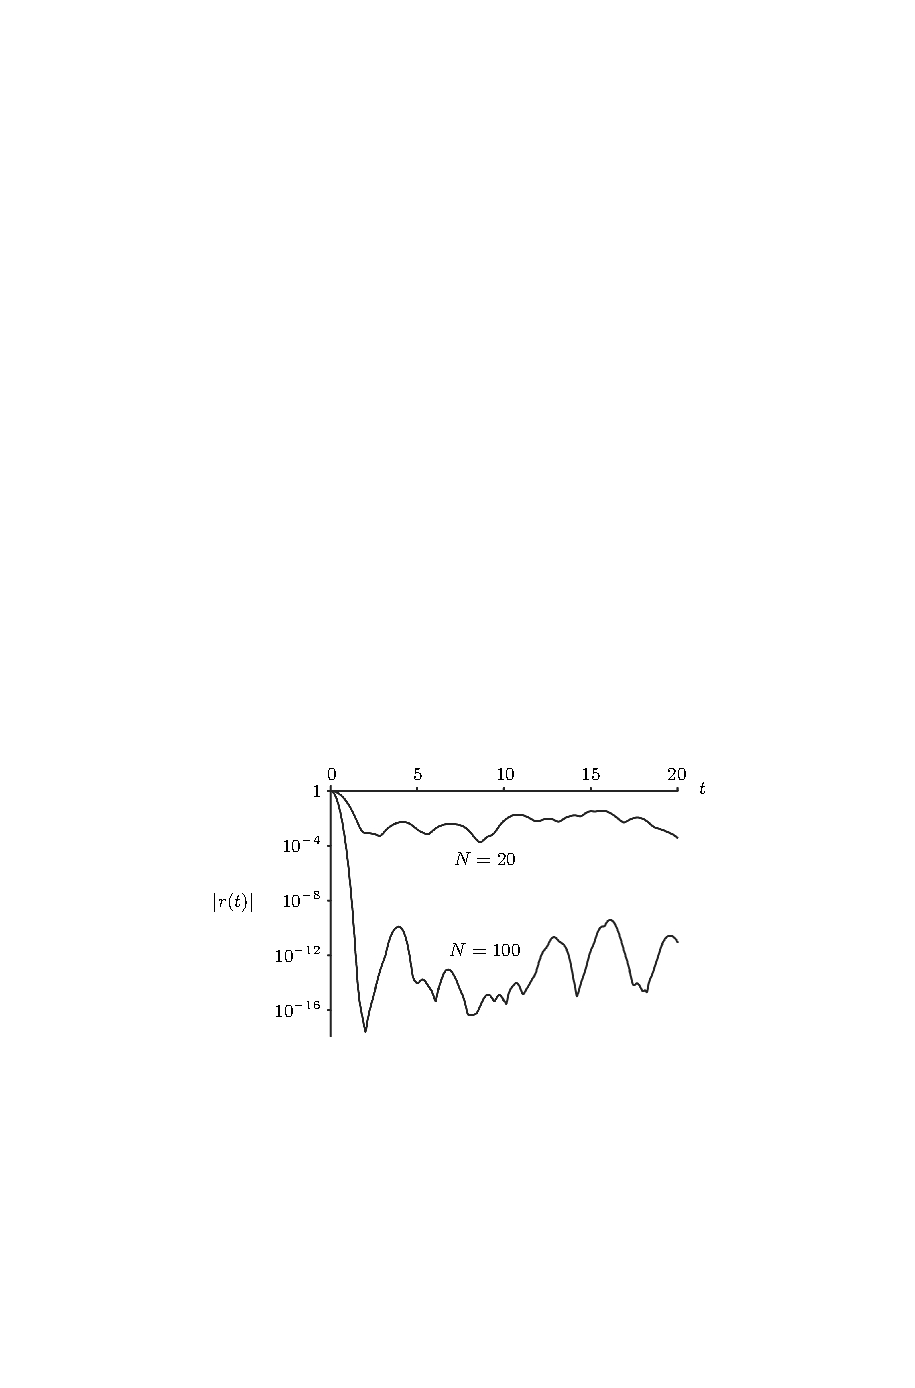
\includegraphics[width=.84\linewidth]{figures/ch02_fig06.pdf}\caption{デコヒーレンス因子$r(t)$［式(2.107)］の絶対値の発展。$N$個の静的な環境スピンの集まりと相互作用する、静的な中心スピン系の干渉項の時間依存性を、異なる二つの値$N=20$、$N=100$について記述する。各環境スピンの初期状態は完全にランダムとし、環境スピンは相互にも、系とも完全に無相関とした。結合は区間$[0,1]$からランダムに選んだ。}\end{figure}

しかし環境スピン数、したがって環境自由度数が有限である限り、デコヒーレンス因子(2.107)が初期値の1へ戻る、特徴的な回帰時間$\tau_{\mathrm{rec}}$が必ず存在することを認識するのが重要である。これは単に、式(2.107)が時間的に周期的な関数の和であることの帰結である。そのような周期関数の和は、それ自体も周期的でなければならない。回帰時間の値は、環境の初期状態と結合$g_i$の分布による。たとえば、環境スピン間に初期相関がない、高度に「非ランダム」な環境の初期状態
\begin{equation}\lvert\Psi(0)\rangle=(a\lvert0\rangle+b\lvert1\rangle)\prod_{i=1}^N\frac1{\sqrt2}(\lvert\uparrow\rangle_i+\lvert\downarrow\rangle_i)\tag{2.111}\end{equation}
という極限で、すべての$i$について$g_i=g$とすると、式(2.107)は

% 原文 p.93
\hypertarget{srcpage:93}{}\label{srcpage:93}
\begin{equation}r(t)=\cos^N(gt)\tag{2.112}\end{equation}
を与える。このデコヒーレンス因子は振動数$g/2\pi$で周期的である。したがって、その絶対値$\lvert r(t)\rvert$が減衰を示すのは$t<\pi/g$の時間だけで、$\tau_{\mathrm{rec}}=\pi/g$の整数倍の時刻に、コヒーレンスの完全な復活が起こる。また環境が、たまたま$\hat E$の固有状態$\lvert n\rangle$の一つから出発する極端な状況では、$r(t)$はまったく減衰せず、したがってデコヒーレンスも起こらない。

現実的な場合、このように高度に秩序立った初期状態と、対称的な系と環境の結合が、関係する可能性は低い。その場合、特徴的な回帰時間$\tau_{\mathrm{rec}}$は通常、きわめて長く、$\tau_{\mathrm{rec}}\propto N!$というPoincaré型になる。現実的だが有限の大きさの巨視的環境では、Zurek\cite{ref009}が最初に指摘したように、$\tau_{\mathrm{rec}}$は宇宙の寿命を超えうる。したがって系からのコヒーレンス喪失が、通常、実際上あらゆる目的に対して不可逆なのは、環境を制御し観測する実際上の能力がないだけでなく、ほぼすべての物理的に現実的な状況で、コヒーレンス回帰の時間尺度が天文学的に大きいからでもある。
